\section{空间直线、平面的垂直}

本节要点:
\begin{itemize}
    \item 掌握异面直线的夹角的定义;
    \item 掌握线面平行的定义;
    \item 掌握线面平行的定理;
    \item 掌握线面平行的性质。
\end{itemize}

~

教材中没有给出异面直线的夹角的明确定义,我们需要领会精神,本质就是通过构造平行线,将异面直线转化为共面直线。所以,所有涉及异面直线夹角的问题,都需要构造平行线,化成共面直线。

本节讨论线面的第二个重点关系,即垂直,依然按照“定义—定理—性质”的步骤理解本节内容。

线面垂直:
\begin{itemize}
    \item 定义:直线和平面内任意直线垂直,注意这里引出的“距离”概念;
    \item 定理:若直线和平面内两条交线垂直,则线面垂直,如下左图;
    \item 性质:若两条直线都和平面垂直,则两条直线平行,如下中图。
\end{itemize}

\begin{figure}[h]
\centering
\begin{minipage}{.32\textwidth}
\centering
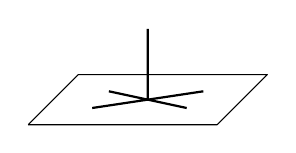
\begin{tikzpicture}[style={x={(-135:0.5)},y={(1cm,0)},z={(0,1cm)}}, line join=round, scale=0.3]
\draw (3,-4,0)--(3,4,0)--(-3,4,0)--(-3,-4,0)--(3,-4,0);
\draw[thick] (1,-2,0)--(-1,2,0) (-1,-2,0)--(1,2,0) (0,0,0)--(0,0,3);
\end{tikzpicture}
\end{minipage}
\begin{minipage}{.32\textwidth}
\centering
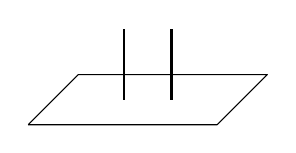
\begin{tikzpicture}[style={x={(-135:0.5)},y={(1cm,0)},z={(0,1cm)}}, line join=round, scale=0.3]
\draw (3,-4,0)--(3,4,0)--(-3,4,0)--(-3,-4,0)--(3,-4,0);
\draw[thick] (0,-1,0)--(0,-1,3) (0,1,0)--(0,1,3);
\end{tikzpicture}
\end{minipage}
\begin{minipage}{.32\textwidth}
\centering
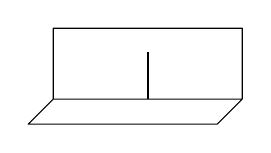
\begin{tikzpicture}[style={x={(-135:0.5)},y={(1cm,0)},z={(0,1cm)}}, line join=round, scale=0.3]
\draw (0,-4,0)--(3,-4,0)--(3,4,0)--(0,4,0)--(0,-4,0)--(0,-4,3)--(0,4,3)--(0,4,0);
\draw[thick] (0,0,0)--(0,0,2);
\end{tikzpicture}
\end{minipage}
\end{figure}

\begin{tcolorbox}
教材对性质的证明使用反证法P153,反复阅读,领会精神!同时注意旁边的框框,它说明了为什么只能用反证法。
\end{tcolorbox}

平平垂直:
\begin{itemize}
    \item 定义:二面角为90°;
    \item 定理:若线面垂直,则平平垂直,如上右图;
    \item 性质:若平平垂直,则垂直于交线的直线构成线面垂直,同如上右图。
\end{itemize}

\begin{tcolorbox}
教材对性质的证明使用二面角的定义P159,反复阅读,领会精神!
\end{tcolorbox}

\begin{tcolorbox}
垂直关系是本章的重点,本节的例5、例7、例8、例10,以及两个性质的证明集中体现了垂直关系的要点,必须反复阅读,领会精神!
\end{tcolorbox}

~

\begin{example}[拓广探索19,难度:$\star $]
如图,在直三棱柱$ABC-A_1B_1C_1$中,$\angle ABC=90^\circ ,AA_1=AB$,求证$A_1C\bot AB_1$。
\end{example}

\begin{figure}[h]
\centering
\begin{minipage}{.49\textwidth}
\centering
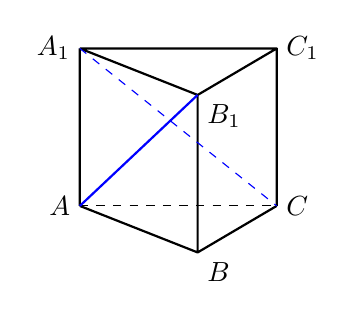
\begin{tikzpicture}[style={x={(-100:0.5)},y={(1cm,0)},z={(0,1cm)}}, line join=round, scale=0.5]
\coordinate[label=left:       {$A$}]   (A)  at (0,0,0);
\coordinate[label=right:      {$C$}]   (C)  at (0,5,0);
\coordinate[label=below right:{$B$}]   (B)  at (2.4,3.2,0);
\coordinate[label=left:       {$A_1$}] (A1) at (0,0,4);
\coordinate[label=right:      {$C_1$}] (C1) at (0,5,4);
\coordinate[label=below right:{$B_1$}] (B1) at (2.4,3.2,4);
\draw[thick] (A1)--(B1)--(C1)--(A1) (A)--(B)--(C) (A)--(A1) (B)--(B1) (C)--(C1);
\draw[dashed] (A)--(C);
\draw[thick,blue] (A)--(B1);
\draw[dashed,blue] (A1)--(C);
\end{tikzpicture}
\end{minipage}
\begin{minipage}{.49\textwidth}
\centering
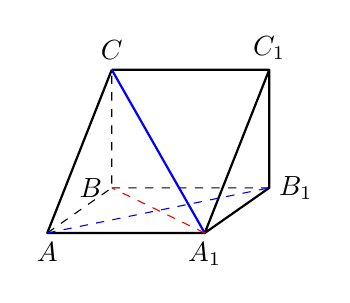
\begin{tikzpicture}[style={x={(-145:0.5)},y={(1cm,0)},z={(0,1cm)}}, line join=round, scale=0.5]
\coordinate[label=left: {$B$}]   (B)  at (0,0,0);
\coordinate[label=below:{$A$}]   (A)  at (4,0,0);
\coordinate[label=above:{$C$}]   (C)  at (0,0,3);
\coordinate[label=right:{$B_1$}] (B1) at (0,4,0);
\coordinate[label=below:{$A_1$}] (A1) at (4,4,0);
\coordinate[label=above:{$C_1$}] (C1) at (0,4,3);
\draw[thick] (C)--(A)--(A1)--(C1)--(C) (A1)--(B1)--(C1);
\draw[dashed] (A)--(B)--(C) (B)--(B1);
\draw[dashed,blue] (A)--(B1);
\draw[thick,blue] (A1)--(C);
\draw[dashed,red] (A1)--(B);
\end{tikzpicture}
\end{minipage}
\end{figure}

解:

原图不容易看,换一下,以$AA_1B_1B$为底,并添辅助线$A_1B$。不难证明线$CB$与面$AA_1B_1B$垂直,于是面$CBA_1$面$AA_1B_1B$垂直,后略。

\begin{tcolorbox}
有时,将立体图形换个角度,有助于发现关键点。
\end{tcolorbox}

~

\begin{example}[拓广探索21,难度:$\star \star $]
如图,在四棱锥$P-ABCD$中,底面$ABCD$为正方形,$PA\bot $底面$ABCD$,$PA=AB$,$E$为线段$PB$的中点,$F$为线段$BC$上的动点。平面$AEF$与平面$PBC$是否相互垂直?如果垂直,请证明;如果不垂直,请说明理由。
\end{example}

\begin{figure}[h]
\centering
\begin{tikzpicture}[style={x={(-145:0.5)},y={(1cm,0)},z={(0,1cm)}}, line join=round, scale=2.5]
\coordinate[label=above:      {$P$}] (P) at (1,0,1);
\coordinate[label=below left: {$A$}] (A) at (1,0,0);
\coordinate[label=below right:{$B$}] (B) at (1,1,0);
\coordinate[label=right:      {$C$}] (C) at (0,1,0);
\coordinate[label=left:       {$D$}] (D) at (0,0,0);
\coordinate[label=above right:{$E$}] (E) at ($(P)!0.5!(B)$);
\coordinate[label=below right:{$F$}] (F) at ($(B)!0.8!(C)$);
\draw[thick] (B)--(P)--(A)--(B)--(C)--(P);
\draw[dashed] (P)--(D)--(A) (D)--(C);
\draw[thick,blue] (A)--(E)--(F);
\draw[dashed,blue] (A)--(F);
\fill[blue!50!white,opacity=0.5] (A)--(E)--(F)--cycle;
\fill[pink!50!white,opacity=0.5] (B)--(C)--(P)--cycle;
\end{tikzpicture}
\end{figure}

解:

大致过程如下:
\begin{align*}
&\because \bigtriangleup APB\text{为等腰直角}\Rightarrow AE\bot PB \\
&\because CB\bot \text{面}APB\Rightarrow CB\bot AE \\
&\therefore AE\bot \text{面}PCB
\end{align*}

\begin{tcolorbox}
动点$F$可以理解为面$AEF$绕着轴$AE$旋转,就容易理解了。
\end{tcolorbox}




